\documentclass[a4paper]{article}

\usepackage[fontset=fandol]{ctex}
\usepackage{amsmath, amssymb}
\usepackage{graphicx}
\usepackage[margin=2.5cm]{geometry}
\usepackage[most]{tcolorbox}
\usepackage{etoolbox}
\usepackage{listings}
\usepackage{hyperref}
\usepackage{booktabs}
\usepackage{subcaption}
\usepackage{float}
\usepackage{tikz}
\IfFileExists{pgfplots.sty}{
    \usepackage{pgfplots}
    \pgfplotsset{compat=1.18}
}{}

\hypersetup{
  colorlinks=true,
  linkcolor=blue!55!black,
  urlcolor=blue!55!black
}

\newtcolorbox{knowledgebox}[1]{
    enhanced, colback=blue!5!white, colframe=blue!75!black, colbacktitle=blue!75!black,
    coltitle=white, fonttitle=\bfseries, title=#1, attach boxed title to top left={yshift=-2mm, xshift=2mm},
    boxrule=1pt, sharp corners, breakable
}

\newtcolorbox{importantbox}[1]{
    enhanced, colback=yellow!10!white, colframe=yellow!80!black, colbacktitle=yellow!80!black,
    coltitle=black, fonttitle=\bfseries, title=#1, sharp corners, breakable
}

\newtcolorbox{warningbox}[1]{
    enhanced, colback=red!5!white, colframe=red!75!black, colbacktitle=red!75!black,
    coltitle=white, fonttitle=\bfseries, title=#1, sharp corners, breakable
}

\newtcolorbox{dialoguebox}[1]{
    enhanced, breakable, colback=green!4!white, colframe=green!45!black, colbacktitle=green!45!black,
    coltitle=white, fonttitle=\bfseries, title=#1, sharp corners
}

\lstset{
    language=Python,
    basicstyle=\ttfamily\small,
    keywordstyle=\color{blue},
    stringstyle=\color{red!60!black},
    commentstyle=\color{green!60!black},
    breaklines=true,
    frame=single,
    numbers=left,
    numberstyle=\tiny\color{gray},
    captionpos=b,
    extendedchars=false
}

\newcommand{\notetitle}{爆款内容是怎么炼成的：Tim 的内容产品、团队复制与商业化方法论}
\newcommand{\notesubtitle}{从表达欲到工业化协作：一场刘润×Tim 访谈里的内容创业课（公式减少优化版）}
\newcommand{\noteauthors}{刘润商学视频整理 \& Codex}
\newcommand{\notedate}{2026年7月2日}
\newcommand{\videochannel}{刘润商学}
\newcommand{\videopublishdate}{2026-04-27}
\newcommand{\videoduration}{01:17:44}
\newcommand{\videourl}{https://www.bilibili.com/video/BV1yeoCBMEv7/}
\newcommand{\videocoverpath}{source.jpg}

\makeatletter
\newcommand{\compacttableofcontents}{%
  \begingroup
  \footnotesize
  \setlength{\parskip}{0pt}
  \renewcommand{\baselinestretch}{0.86}\selectfont
  \renewcommand*\l@section[2]{\@dottedtocline{1}{0em}{2.4em}{\bfseries ##1}{\bfseries ##2}}%
  \renewcommand*\l@subsection{\@dottedtocline{2}{1.6em}{3.2em}}%
  \tableofcontents
  \endgroup
}
\makeatother

\begin{document}

\begin{titlepage}
\centering
\vspace{1.0cm}
{\huge\bfseries \notetitle\par}
\vspace{0.45cm}
{\Large \notesubtitle\par}
\vspace{0.75cm}
{\large \noteauthors\par}
\vspace{0.25cm}
{\large \notedate\par}
\vspace{1.0cm}

\includegraphics[width=0.82\textwidth,height=0.45\textheight,keepaspectratio]{\videocoverpath}\par

\vfill
\begin{tcolorbox}[width=0.9\textwidth, colback=black!2!white, colframe=black!60, sharp corners]
\textbf{视频作者/频道}：\videochannel\par
\textbf{发布日期}：\videopublishdate\par
\textbf{视频时长}：\videoduration\par
\textbf{视频链接}：\href{\videourl}{\nolinkurl{\videourl}}\par
\textbf{材料依据}：Bilibili 字幕、视频封面、关键时间点抽帧与机制化重绘图。
\end{tcolorbox}
\end{titlepage}

\compacttableofcontents
\medskip

\section{导言：从访谈到内容创业课}

这篇 PDF 的答案先放在开头：爆款内容的炼成，靠的是创作者把个人表达欲转化为可被传播的内容产品，再用工业化协作、自由化管理、OKR 与商业化闭环持续放大；真正的底层目标，是长期输出能打动人心的作品。

刘润与 Tim 的这场访谈，表面上在聊“影视飓风为什么能做爆款”。更深一层，它在回答一套内容创业系统问题：创作者、内容、组织、管理、商业和愿景怎样互相承接。

\begin{knowledgebox}{核心概念图}
本文使用六个概念组织全篇。第一，\textbf{创作者表达}指个人把兴趣、压力、自学和长期输出转成作品的能力，对应第一章。第二，\textbf{内容产品}指一条内容同时具备选题、叙事、知识、情绪、节奏和传播设计，对应第二章。第三，\textbf{工业化协作}指把个人判断交给编导、制片、摄影、技术、产品等角色共同承接，对应第三章。第四，\textbf{自由化管理}指路径自主、目标清晰、结果可检验的管理方式，对应第四章。第五，\textbf{商业化闭环}指广告、商业服务、电商、创意权和观众信任之间的可持续关系，对应第五章。第六，\textbf{使命牵引}指“无限进步”“让中国人燃起来”和“输出打动人心的作品”对长期选题、人才和商业模式的约束，对应第六章与总结。
\end{knowledgebox}

因此，本文的关键问题应按六层结构理解：

\begin{enumerate}
  \item \textbf{人}：Tim 的表达欲、自学和输出纪律怎样成为内容创业的原材料。
  \item \textbf{内容}：爆款怎样通过快乐、知识、共鸣和节奏触发传播。
  \item \textbf{组织}：个人创作方法怎样进入百人团队与工业化协作。
  \item \textbf{管理}：自由化管理和 OKR 怎样让创意自由接受结果检验。
  \item \textbf{商业}：内容公司怎样让商业资源、观众信任和创作者伦理共同成立。
  \item \textbf{愿景}：公司化之后，创作者身份、使命和未来目标怎样牵引长期作品力。
\end{enumerate}

\begin{importantbox}{全文主线}
本文按“人 -> 内容 -> 组织 -> 管理 -> 商业 -> 愿景”的顺序重组访谈。读者先看到创作者能力从哪里来，再看到爆款内容如何设计，随后进入团队复制、管理指标、商业伦理和长期使命。这样的结构让访谈从人物故事变成一套可复盘的内容创业课。
\end{importantbox}

文中保留了关键时间点、对话片段、视频帧和教学化图表。本版减少临时公式，优先用清晰段落、列表和表格解释访谈中的经验判断；只有在公式能表达约束、阈值或可复用判断关系时才保留形式化表达。读者使用本文时，应把它看作一份“从访谈提炼方法”的学习笔记，逐字转录不属于本文目标。

\section{从表达欲到内容创业：爆款的原材料是什么}

本章先给结论：Tim 后来能把内容做成近 4000 万粉丝规模的事业，早期关键因素包括表达欲、孤立环境、自学能力、长期输出、赛道扩宽、平台窗口和低资源创业。它们共同把一个 1996 年出生的创作者推向内容公司化。读者真正需要抓住的是顺序：表达欲提供驱动力，孤立环境带来自我审视，自学和长期输出形成能力，赛道扩宽与平台窗口放大能力，低资源创业检验能力。

\subsection{起点：普通人、压力与责任感}

访谈开场给了两个容易被同时忽略的事实：一方面，Tim 被介绍为 1996 年出生、全网粉丝近 4000 万、影视飓风自 2015 年以来做出多条爆款视频；另一方面，他对自己的定位很朴素，认为自己和大家一样，会吃饭喝水，也会做错误决定。这个开场很关键，因为它把“神秘的头部 UP 主”拉回到一个具体的人：他有内容能力，也有经营压力。\footnote{源时间：00:00:00--00:01:36}

\begin{importantbox}{本章主张（源时间：00:00:54--00:01:36）}
Tim 的创作者能力是一条积累链：先有持续表达的内在冲动，再有孤立环境里的自学和高频输出，随后通过更宽赛道和平台窗口被放大，最后在低资源条件下进入创业状态。读者学习这一章时，应把“经历”看作要素组合，避免把人物故事当成励志段子。
\end{importantbox}

刘润把 Tim 从“UP 主”提升到“创业者”视角时，Tim 给出的规模信息很实在：他从高一开始做视频，先一个人做了四年，后来有小团队，2018 年真正意义上回国创业；团队从三个人、始终没有收益，增长到约 110 人，并且没有真正意义上的融资。\footnote{源时间：00:01:04--00:02:28} 这意味着第一章要回答的核心问题可以改写为：一个能持续输出的人，怎样一步步获得承担公司成本的能力。

这里的“责任感”具体指向成本与现金流。110 人团队意味着每月百万级成本，一年需要上千万营收支撑。创作者一旦公司化，作品就同时承载三层责任：观众要看好内容，员工要有生活，商业系统要持续运转。这个事实会在后续章节展开；本章先把源头讲清楚：承担压力之前，Tim 先练出了表达和学习的底层能力。

\subsection{英国经历：孤立环境怎样逼出自学与表达}

Tim 的英国高中经历不能被写成轻飘飘的“海外成长故事”。源材料里有几件很硬的事实：他在国内成绩不好，初中阶段沉迷游戏；父母把他送到英国私校后，学校里只有他一个中国人；刚到时英文沟通困难，前两个礼拜因为不敢开口问老师而没有被子，只能睡在裸床上；他还提到被乌克兰同学欺负和霸凌的经历。\footnote{源时间：00:02:36--00:05:24}

\begin{dialoguebox}{表达能力与沟通意愿（源时间：00:04:58--00:05:02）}
Tim：现在因为接触的人多了，可能会更开朗一点，更愿意表达；表达能力还可以，日常沟通意愿没有那么强。
\end{dialoguebox}

这段话的教学价值很高：表达能力和日常沟通意愿是两件相关却独立的事。一个人可以内向，也可以通过作品表达得很强。对内容创作者来说，镜头、文字、剪辑、教程、漫画、评测都可以成为表达媒介；社交场合里的健谈不属于创作能力的必要条件。

\begin{figure}[htbp]
  \centering
  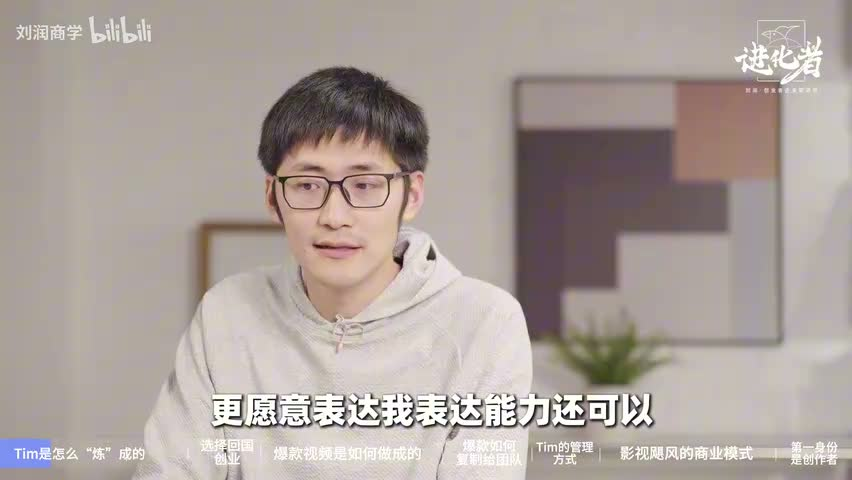
\includegraphics[width=0.70\linewidth,height=0.30\textheight,keepaspectratio]{figures/selected/frame_00-05-00_expression_ability.jpg}
  \caption{Tim 早期自我定位：表达能力已经显现，表达欲来自更长时间的环境压力、自学和作品训练。\protect\footnotemark}
  \label{fig:section01-expression-ability}
\end{figure}
\footnotetext{视频画面时间区间：00:04:58--00:05:02}

\begin{warningbox}{别把痛苦写成万能因果（源时间：00:04:21--00:06:10）}
孤立、被欺负、没被子这些经历本身不会自动生成创作能力。真正发生作用的因素，是孤立环境迫使人长时间审视自己，随后把兴趣、情绪和问题意识转成可发布的作品。痛苦只提供压力；表达欲和自学行动才提供产出。
\end{warningbox}

Tim 后来把那段时间称为“自我思维萌芽”的机会：一个人会花很长时间审视自己、思考人生、冒出很多点子。\footnote{源时间：00:05:57--00:06:13} 这正是“孤立带来自我审视”的具体含义。注意力被迫向内聚集后，会产生大量未成形想法；这些想法需要后续写作、剪辑和发布来完成外化。

\subsection{从小说、漫画到视频：长期输出如何训练内容肌肉}

Tim 的早期输出路径很连续：先写游戏同人和玄幻小说，再与读者合作漫画，随后转向动态影像，开始自学 After Effects 和 Premiere。最值得注意的是输出强度。他说自己写小说时保持每天约 8000 字，持续两年，最终写了 140 多万字；当时作品发在贴吧，确实有一批读者跟着看，粉丝约 1 万多。\footnote{源时间：00:06:13--00:07:08}

“140 多万字”具有训练含义。对于创作者训练而言，它意味着至少三件事：第一，能长期坐下来产出；第二，能承受早期作品粗糙；第三，能在反馈中维持下一次更新。很多人把内容能力理解成灵感，实际阅读 Tim 的经历会发现，它更接近肌肉训练：

\begin{itemize}
  \item \textbf{输入要足够密}：他持续看教程、学软件、研究设备和视频表达。
  \item \textbf{输出要足够频繁}：小说、漫画、教程、视频更新共同提供了高频练习。
  \item \textbf{反馈要足够真实}：贴吧读者、优酷观众、学校宣传任务和 B 站播放量，都在告诉他哪些表达有效。
\end{itemize}

这样写比临时公式更省读者精力：创作者能力增长的关键，不在符号定义，而在“持续输入、持续输出、持续反馈”这三个可操作动作同时发生。

漫画阶段补上了第二种训练：把文字故事交给画面表达。Tim 与一位会画画的读者合作，把玄幻小说画成漫画，作品在网上发布，也获得过一些杂志渠道的反馈。\footnote{源时间：00:07:09--00:07:46} 这一步让他意识到，自己更想做动态的东西。于是，他开始接触 AE、Premiere，自学视频软件。

自学阶段的强度同样惊人。Tim 说自己每天保持 14 到 15 小时学习，大量摄入 AE 知识和视频知识，并且看的教程全是英文。兴趣带动学习，英语水平随之快速提升。到第二年，他已经进入学生会，负责学校宣传相关视频工作。\footnote{源时间：00:07:46--00:08:41} 这里有一个反直觉点：语言学习的突破，来自“为了做视频必须看英文教程”的真实任务驱动。

\begin{knowledgebox}{什么叫“内容肌肉”？}
内容肌肉指的是创作者把输入转成作品的稳定能力。它包括选题、叙事、技术、发布节奏和接受反馈的耐受力。小说训练坚持力，漫画训练画面化表达，视频训练技术和节奏；三者叠加后，创作者才有机会把表达欲变成可传播内容。
\end{knowledgebox}

接下来，Tim 又把自学变成教学。他在优酷上发布教程，向国内用户分享 AE 操作和效果制作。为了跟上教学速度，他需要用更高强度去学习，形成“看、学、做、教、更新”的循环。他说自己从写小说转向做视频后，做不到每天更新视频，也可以每周更新，并且一直坚持多年。\footnote{源时间：00:09:35--00:10:27} 这就是长期输出 reps：一次作品可能偶然，一周一更多年则会塑造能力结构。

\subsection{赛道扩宽：从后期教学到影视设备评测}

2017 到 2018 年左右，有粉丝建议 Tim 做硬件设备评测，不再只做后期教学。他开始做影视设备、相机、拍摄和灯光评测，并由此第一次意识到“赛道对于一个人的空间有多大”。源材料里说得很具体：后期教学相对窄，进入前期和设备评测后，市场明显更大；播放量从几百上升到几千，有时能破万。\footnote{源时间：00:10:30--00:11:04}

赛道可以理解为内容的“可触达人群半径”。同样的表达能力，如果只服务很窄的软件教程圈层，增长上限会很快到来；如果扩展到设备、拍摄、灯光、相机评测，受众从“学后期的人”扩展为“关心影像创作和消费设备的人”。半径一变，反馈量、商业可能性和平台推荐空间都会变。

这一步还叠加了平台时机。Tim 提到那时 B 站开始慢慢有起色，第一波大众化浪潮开始起来，他的账号也随着 B 站整体大流被推向更多人。\footnote{源时间：00:11:04--00:11:16} 平台窗口不能替代个人积累，却能放大已有能力。若没有前面的写作、视频、剪辑、评测积累，窗口打开也抓不住；若没有窗口，早期能力也更难迅速变成规模影响力。

这一节给创作者的启发很直接：能力和赛道要一起看。只问“我会什么”还不够，还要问“这个能力放在哪个问题域里，能触达更大人群”。Tim 从后期教程走向影视设备评测，本质上就是从工具教学扩展到影像消费和创作生态。

\subsection{大学阶段：自我导向、设备投入与相机评测学徒期}

赛道扩宽之后，Tim 在英国大学阶段完成了一个关键桥接：他把自学兴趣推向市场化创作场景。源材料里，他谈到自己读的是电影相关专业，但课堂带来的直接帮助有限；更重要的是每天自己出去走、自己拍、自己学，把注意力放在真正感兴趣的影像问题上。\footnote{源时间：00:11:16--00:12:37。} 这说明他的学习方式很早就带有强烈自我导向：学校提供身份和环境，能力增长主要来自持续项目、设备实践和外部反馈。

资源配置也很极端。Tim 提到当时每月生活费大约 400 英镑，他会把大量钱花在设备上，甚至为了买器材压缩饮食开销，还经历过靠 Huel 等代餐解决吃饭问题的阶段。\footnote{源时间：00:12:37--00:14:09。} 这个细节不该被浪漫化。它真正说明的是，早期创作者常常要用非常有限的资源做艰难取舍：吃得更好、生活更稳，和更快积累设备、作品与经验，短期内会互相挤压。

随后出现的相机评测学徒期，把他的自学推进到行业现场。Tim 主动联系一位大型相机评测创作者，在没有报酬的情况下帮忙做拍摄、后期和相关工作；接下来大约两年，他在伦敦高频参与工作，同时维持自己 B 站账号更新。\footnote{源时间：00:14:09--00:17:26。} 这段经历补上了“为什么后来能做设备评测”的中间因果：他接触了真实评测工作流，见到了更专业的创作者生产方式，也在双线输出压力下训练了速度和可靠性。

\begin{knowledgebox}{自我导向学习}
自我导向学习指学习者自己决定学什么、为什么学、怎样验证结果。Tim 的例子里，课堂只是背景；真正形成能力的是设备实践、免费协作、相机评测现场和持续发布。它像在真实厨房里学做菜：教材能给概念，出餐压力、顾客反馈和师傅要求会逼出手上功夫。
\end{knowledgebox}

\subsection{回国创业：机会窗口与低资源起步}

大学后期，Tim 面前出现了一个典型机会成本选择：申请南加大硕士，或回国创业。他最终选择回国，因为创业是他更想做的事情。他回头判断，如果当时去读硕士，后来的很多事情都不会发生；B 站对影视飓风来说，关键红利期集中在 2018 到 2019 年这个周期。\footnote{源时间：00:17:26--00:18:00}

\begin{knowledgebox}{机会成本与平台窗口}
机会成本指为了选择 A 而放弃 B 的价值。在这里，读硕士的价值可能是学历、系统训练和海外路径；回国创业的价值是抓住 2018--2019 年 B 站大众化增长窗口。平台窗口像潮水，个人准备度像船；船没有准备好会被浪打翻，潮水过去后再好的船也很难获得同样速度。
\end{knowledgebox}

回国后的启动条件并不优越。Tim 说，2019 年很多人还不认为在 B 站开账号可以叫创业，外界更容易把他们看成“小孩子过家家”。他们在园区租了一个很破的食堂，回来后真的没钱，贷款 6 万元，刷油漆也自己刷，几位伙伴一起干。\footnote{源时间：00:18:00--00:18:57} 这就是低资源启动能力的具体含义：现金少、条件差、外界不理解，团队仍然要把有限资源转成可发布作品。

低资源启动的关键，是观察一个团队在现金少、外界不理解、没有融资、没有成熟组织结构时，能不能把所有可用资源都转成作品。破食堂、6 万贷款、自刷油漆这些细节说明，影视飓风早期并没有一套成熟公司系统可用；他们先有的是创作惯性、伙伴协作和对平台窗口的判断。

把第一章串起来看，Tim 的路径可以压缩成一条链：英国孤立带来自我审视，小说和漫画把想法变成作品，AE/Premiere 自学带来视频表达能力，每周更新形成输出纪律，设备评测打开更宽赛道，B 站 2018--2019 年窗口放大账号增长，回国后用 6 万贷款和几位伙伴把内容账号推进到创业状态。后面从三人无收益走到 110 人团队，靠的就是这条链逐步积累出的能力底座。

\subsection{本章小结}

本章的核心判断是：爆款内容的第一块原材料，是一个能持续表达、持续学习、持续发布的人。Tim 的早期经历提供了六条可迁移经验：

\begin{itemize}
  \item 表达欲与外向性格不能画等号；内向的人也可以通过作品建立强表达。
  \item 孤立环境只能提供压力和反思时间，真正产生能力的是后续自学和作品输出。
  \item 140 多万字小说、漫画合作、AE/Premiere 自学和每周视频更新，共同训练了坚持力、叙事能力、技术能力和反馈耐受力。
  \item 赛道决定增长半径；从后期教学走向影视设备评测，扩大了受众、反馈和商业空间。
  \item 平台窗口会放大已有能力；2018--2019 年 B 站大众化浪潮对影视飓风极其关键。
  \item 低资源创业考验的是把有限现金、伙伴协作和创作惯性全部转成作品的能力；6 万贷款和破食堂起步，是内容公司化之前的真实地面。
\end{itemize}

下一章进入“爆款机制”：当一个创作者已经具备持续输出能力，真正决定频道高度的，就变成选题、情绪、知识、共鸣和节奏怎样共同触发传播。
\section{爆款机制：从“能火”到“值得传播”}

本章先给结论：爆款内容的表层价值是单条播放量好看，更深层价值是改变频道高度、受众半径、商业议价权和团队信心。Tim 在访谈里给出的核心方法，可以直接写成四个判断点：快乐让人愿意看，知识让人觉得值，共鸣让人愿意把自己放进内容里，节奏让内容被看完并被记住。\footnote{源时间：00:33:59--00:35:48。}

\begin{importantbox}{本章主张（源时间：00:18:57--00:19:19）}
“只有爆款会决定频道的高度”这句话，应理解为内容公司的增长杠杆：常规内容维持关系，爆款内容打开新圈层；常规内容积累信任，爆款内容改变外部认知；常规内容让老用户留下，爆款内容让更多陌生人第一次认识你。
\end{importantbox}

\begin{figure}[htbp]
  \centering
  
\includegraphics[width=0.70\linewidth,height=0.30\textheight,keepaspectratio]{figures/selected/frame_00-18-58_burst_decides_channel_height.jpg}
  \caption{Tim 对爆款价值的中心判断：爆款决定频道高度。\protect\footnotemark}
  \label{fig:section02-burst-height}
\end{figure}
\footnotetext{视频画面时间区间：00:18:57--00:19:01。}

\subsection{爆款决定频道高度：第一次从 20 万到 45 万}

Tim 回顾 2019 年以前的账号增长时，给出了一组很硬的事实：从 2014、2015 年开始积累，到 2019 年账号才刚到 20 万粉；他已经拼尽全力。真正的转折，来自父亲对爆款价值的提醒：很多博主靠一个视频爆火获得快速增量，影视飓风也必须从底层思考什么内容能打动人心。\footnote{源时间：00:18:57--00:19:47。}

这个提醒很重要，因为它把“爆款”从运气问题改写成战略问题。若只把爆款理解成平台随机推荐，创作者只能等待；若把爆款理解成对人心、议题、故事、投入和节奏的系统设计，创作者就能主动提高命中率。Tim 后来强调，每一条都要当成爆款去做，没爆只是结果没发生，制作时必须用爆款标准要求自己。\footnote{源时间：00:33:24--00:33:47。}

2019 年 1 月发布的“20 万粉丝的博主能赚多少钱”，成为影视飓风第一次真正意义上的爆款。它讲的核心并不华丽：公司当时十几个人，一年约 40 万毛利，人员成本发完几乎不剩；频道广告价值还没起来，主要收入来自 TVC 广告；商业与理想之间存在真实冲突。\footnote{源时间：00:20:02--00:21:19。} 这条视频一周内把账号从 20 万粉推到 45 万粉，让团队第一次切身感受到爆款的力量。

\begin{dialoguebox}{第一次爆款的高信号信息（源时间：00:20:02--00:21:19）}
\textbf{Tim}：2019 年 1 月做了“20 万粉丝的博主能赚多少钱”，客观讲了商业结构；公司已经有十几个人，一年只有约 40 万毛利，工资一发基本不剩。

\textbf{Tim}：那条视频一周内把我们从 20 万粉做到 45 万粉，是人生中第一次真正意义上的爆款。
\end{dialoguebox}

这条视频为什么会传播？第一，它触碰了当时很隐晦的议题：博主到底怎么挣钱。第二，它把毛利、人员成本、广告来源和焦虑摊开，商业结构呈现得足够具体。第三，它把许多创作者共同面对的问题讲出来：想做理想内容，也要面对公司增长和现金流。观众分享它，表层原因是数字刺激，深层原因是它给出了行业背后的真实结构。

\subsection{题材策略：从圈层内容走向更大议题}

第一次爆款之后，影视飓风开始主动扩宽议题。Tim 说，团队从单独的影像评测，转向社科、人文、大众意义上的影像、电影幕后、电影仿拍和科技评测；科技方向也从专业影视设备扩展到相机、手机等更大众的产品。\footnote{源时间：00:21:56--00:22:41。}

这里有一个容易被忽视的增长原理：内容题材决定潜在受众半径。专业影视设备评测面对的是较窄圈层；iPhone 评测天然连接更大的讨论场，因为苹果发布会本身就像数码领域的公共事件。Tim 把 iPhone 称作“数码春晚”级别的产品，意思是它自带大规模注意力；若内容质量足够，创作者就能承接苹果这一议题带来的广泛讨论。\footnote{源时间：00:22:18--00:22:39。}

同样的逻辑也出现在放气球项目里。2020 年初，团队把相机随气球送到三四万米高空。这个项目不挣钱，属于纯粹项目，却形成了明显的破圈传播。刘润提到自己平时很少刷 B 站，也看到了这条内容；这说明它跳出了影视设备圈层，进入更广泛的“普通人也想看不可思议事情发生”的注意力空间。\footnote{源时间：00:23:54--00:24:32。}

\begin{knowledgebox}{议题半径}
议题半径指一个选题天然能触达的人群范围。影视设备评测的半径主要覆盖影像创作者；iPhone 评测覆盖数码用户、普通消费者和平台公共讨论；高空气球覆盖好奇心、冒险感和视觉奇观。爆款选题通常会把专业能力放进更大的公共议题里，让专业不再只服务小圈层。
\end{knowledgebox}

Tim 的表达更接近一个双层结构：常规内容用来保证更新、维持互动、和老粉丝交朋友；爆款内容需要暂时跳出老粉丝视野，去看更大的议题，结交更广泛的新朋友。\footnote{源时间：00:24:48--00:25:00。} 对内容公司来说，常规内容是底盘，爆款内容是增量发动机，两者共同构成账号增长系统。

这个阶段也埋下了管理问题。Tim 提到，放气球之后的 2021 年创业故事视频更完整地讲过公司痛苦：人员增加带来层级关系，员工会因为许多问题得不到处理而难受，他自己也不清楚怎样给大家画目标；公司文化没有搭好，短期事务不断挤压深层问题，沟通又大量停留在微信里，信息差随之堆积。\footnote{源时间：00:25:00--00:26:02。} 这段经历是后文 OKR、知识库、反馈处理和自由化管理的前情：个人爆款经验一旦进入组织规模，管理工具就会从可选项变成必需品。

\subsection{生产策略：把长期沉淀压缩成高密度故事}

打铁花案例把“爆款怎样生产”讲得更具体。团队最初看到非遗宣传，只是觉得画面好看，心里留下一个“这是中国人的烟花”的种子；后续创意会上反复讨论，判断如何细化，适合哪些商业合作，能否引入甲方投入。等到品牌方表达兴趣，团队开始执行。\footnote{源时间：00:26:22--00:27:07。}

执行层面，影视飓风采用编导和制片匹配制。编导负责有趣创意，制片负责项目执行、资金管控和周期管理；摄影、技术等专职人才再进入动态项目组。Tim 把这种方式视为把影视行业流程放进自媒体流程，用来减少杂事干扰、报销拖累、周期失控和临近交付时的大翻车。\footnote{源时间：00:27:07--00:28:12。} 第三章会继续讲组织复制；本章先关注它对爆款生产的意义：好创意需要工业化承接，否则高投入项目很容易在执行中塌掉。

Tim 随后提出一个很有价值的概念：“精力偷取理念”。他的意思是，自然风景之所以美，是大自然用千万年沉淀出来的结果；非遗传承人一辈子投入某项技艺，创作者用几分钟视频讲述他的一生，天然具备浓缩感和出彩可能。相比从零编一个故事，拍摄已经沉淀了很久的人、物和景，能把外部长期投入压缩给观众。\footnote{源时间：00:29:23--00:29:53。}

\begin{importantbox}{“精力偷取理念”的准确理解}
这里的“偷取”指影像创作者选择已经被时间、技艺、自然或人生经历深度打磨过的对象，再用拍摄、剪辑和叙事把它压缩成观众能感知的高密度故事。自然景观、非遗传承人、特殊工程、科学项目都适合这种逻辑；尊重原对象、讲清来源和保留人物尊严，是这套方法的伦理底线。
\end{importantbox}

这个概念也解释了自媒体生产的“死亡三角”：原创、频率和质量很难同时拉满。团队化可以提高效率，题材本身仍需要时间沉淀。打铁花的优势正在于，传承人和技艺已经积累了很久，影视飓风要做的是把故事讲好，并用高速摄影机和特殊影像视角呈现它。最终，这条内容获得几百万到上千万级传播，成为有商业因素在内、传播仍然很强的大爆款。\footnote{源时间：00:30:04--00:30:59。}

\subsection{商业协同：甲方买的是共同追梦的过程}

直升机航拍案例说明，商业合作也可以成为爆款资源。Tim 提到，国内很少有人做直升机航拍，团队认为这是很有意思的点子，于是和甲方沟通。英特尔买下这个点子，团队进行全国航拍，再用对方电脑完成编辑制作；项目为账号带来很高增量。\footnote{源时间：00:31:02--00:31:20。}

这个案例的关键在于合作方式。Tim 说，他们和甲方的关系很有意思，更像带着甲方一起追梦、一起实现有趣的东西；甲方买到的是整个过程，产品从过程中被带出，曝光只是结果之一。\footnote{源时间：00:31:44--00:32:07。}

这给商业内容划出了一条高标准路径：品牌资源服务故事，故事承载品牌价值，观众看见的是项目本身的不可思议和完成过程。若内容只剩产品露出，观众会迅速识别广告味；若品牌只是被藏起来，甲方价值无法实现。优秀商业内容要在三者之间达成平衡：

\begin{itemize}
  \item 观众看到的首先是有价值、有情绪、有记忆点的内容。
  \item 甲方获得的不止是镜头露出，还包括参与实现高难度项目的品牌角色。
  \item 创作者保留内容判断，让商业资源变成作品完成度的一部分。
\end{itemize}

\begin{warningbox}{爆款商业内容的风险}
商业资源能放大项目，也会放大信任风险。若项目只服务甲方，观众会把它识别为硬广；若创作者只追求视觉奇观，成本可能失控；若品牌角色讲不清，甲方会怀疑投入回报。爆款商业内容必须同时回答三个问题：观众为什么愿意看，甲方为什么愿意买，创作者为什么愿意把信用押上去。
\end{warningbox}

Tim 也坦诚，大的爆款很多仍需要他亲自操刀。团队工业化可以解决产能，创意、真心和个人价值投射更难复制；超级爆款常常需要创作者本人投入经验、天赋和长期经历。\footnote{源时间：00:32:10--00:33:20。} 这指出了爆款生产的两层结构：团队能承接复杂执行，核心创意判断仍要有人负责。

\subsection{四特质模型：快乐、知识、共鸣、节奏}

Tim 总结爆款时，提出通常具有四个特质：快乐、知识、共鸣、节奏。它们分别对应观众“愿意转发”的四种心理动因。\footnote{源时间：00:33:59--00:35:48。}

\begin{figure}[htbp]
  \centering
  
\includegraphics[width=0.86\linewidth,height=0.42\textheight,keepaspectratio]{figures/generated/fig_burst_four_traits_model.pdf}
  \caption{爆款内容四特质：快乐、知识、共鸣、节奏共同制造传播欲。教学化生成图，综合自 00:33:59--00:35:48。}
  \label{fig:section02-four-traits}
\end{figure}

快乐天然具备传播性。搞笑片段、轻松表达、意外反差和幽默解构，会让观众想分享给家人和朋友。知识提供认知价值。观众把一条内容转给别人，常常因为它能帮到身边的人，或者它表达了自己认可的价值观。共鸣更难，因为它要求内容真实触及人的经历和情绪，不能只靠矫饰的作文腔。节奏决定观众是否愿意一直看下去，也决定情绪峰值能否在正确时刻释放。\footnote{源时间：00:34:39--00:35:41。}

可以把四特质进一步写成一个简化检查表：

\begin{table}[htbp]
  \centering
  \caption{爆款四特质的选题检查表}
  \label{tab:section02-four-traits-checklist}
  \begin{tabular}{lll}
    \toprule
    特质 & 核心问题 & 常见表现 \\
    \midrule
    快乐 & 观众会不会带着轻松感分享？ & 幽默开场、反差、解构自己、可转述笑点 \\
    知识 & 观众是否获得新尺度或新信息？ & 数据、原理、行业内幕、可视化解释 \\
    共鸣 & 观众能否把自己放进故事？ & 梦想、压力、真实经历、共同参与感 \\
    节奏 & 信息和情绪是否在正确时刻释放？ & 伏笔、停顿、加速、慢收尾、音乐控制 \\
    \bottomrule
  \end{tabular}
\end{table}

四特质之间存在组合关系。只有快乐，内容可能轻快却很快被忘掉；只有知识，内容可能有用却缺少主动传播动力；只有共鸣，内容可能感人却拖沓；只有节奏，内容可能流畅却缺少真正可记住的价值。爆款的难点在于多项同时成立，并且服务同一个主故事。

\subsection{卫星案例：先同步，再引领}

卫星视频是 Tim 用来解释四特质的标准案例。开场先用幽默把观众吊住：朋友邀请做卫星，用纸板画图，讲预算和团队不懂卫星的窘态，把自己放在普通人的位置上。Tim 强调，互联网表达的本质包含解构，创作者要不断解构自己；以过高姿态开场，观众很难进入。\footnote{源时间：00:35:54--00:36:41。}

接着进入知识层。视频解释卫星到底有多高：空间站约 400 公里，东方红卫星在 500 多公里轨道上，北斗卫星在 32000 公里量级，天问一号火星探测器又在更远的尺度上。它把普通人缺少直觉的距离，用比例和层级呈现出来，让观众拿到一个能复述的新尺度。\footnote{源时间：00:36:41--00:37:24。}

然后进入共鸣。太空影像本身已经震撼，Tim 又把粉丝梦想、屏幕亮起、共同参与感紧接着释放出来，让观众意识到自己参与了一件超出日常尺度的事情。这个顺序很关键：太空影像先给宏大感，粉丝梦想随后点燃个人连接，免费午餐项目和结尾沉思再把情绪往下压，形成更长的回味。\footnote{源时间：00:37:30--00:38:53。}

节奏是最后的控制手段。Tim 提到，结尾选择放慢，谈“如果宇宙的终点是确定的，重要的是过程”。这种慢收尾让观众有反应时间，传播欲反而更强。刘润把这一点连接到演讲和脱口秀里的“先同步后引领”：先同步观众节奏，再带着观众往前走。\footnote{源时间：00:38:14--00:39:37。}

\begin{knowledgebox}{先同步后引领}
“同步”指先进入观众已有的节奏和理解水平，例如用幽默、自嘲、常识问题或具体场景降低门槛；“引领”指在观众已经跟上后，把他们带到更高信息密度、更深情绪或更远视野。演讲可以根据现场反馈动态调节，视频缺少实时反馈，因此更需要未完成版本测试、旁观朋友反应和剪辑节奏校准。
\end{knowledgebox}

Tim 的验证方法也很具体：他会把未完成版本给大量朋友看，站在旁边观察反应；如果感觉“不对”，就说明节奏出了问题。视频创作无法像现场演讲那样实时感知观众，提前测试就变成替代反馈机制。这个动作很朴素，却直接对应爆款的第一性原理：传播发生在观众心里，创作者必须在发布前尽量接近真实观众反应。\footnote{源时间：00:39:41--00:40:28。}

\begin{figure}[htbp]
  \centering
  
\includegraphics[width=0.82\linewidth,height=0.38\textheight,keepaspectratio]{figures/generated/fig_creator_flywheel.pdf}
  \caption{创作飞轮：选题假设、投入、发布、复盘、沉淀和下一轮拷问共同提高爆款命中率。教学化生成图，综合自 00:22:40--00:22:47、00:33:24--00:33:47 与 00:39:41--00:40:28。}
  \label{fig:section02-creator-flywheel}
\end{figure}

\subsection{本章小结}

本章把 Tim 的爆款方法拆成六个层次：

\begin{itemize}
  \item 爆款决定频道高度。影视飓风第一次真正爆款，把账号从 20 万粉推到 45 万粉，让团队看见单条内容改变增长曲线的力量。
  \item 真实议题更容易破圈。“20 万粉丝博主能赚多少钱”抓住商业透明度和理想冲突，iPhone 评测、高空气球等项目则借助更大的公共议题扩大受众半径。
  \item 高密度故事来自长期沉淀。自然景观、非遗传承人和特殊工程已经包含时间投入，创作者通过影像把它压缩给观众。
  \item 商业资源可以成为作品资源。优秀商业合作让甲方参与实现高难度项目，产品价值从故事过程中自然显现。
  \item 四特质构成爆款检查表。快乐让人想分享，知识让人觉得有用，共鸣让人被击中，节奏让人愿意看完并在关键时刻释放情绪。
  \item 节奏需要测试和校准。视频没有现场演讲的即时反馈，未完成版本测试、朋友反应和剪辑调整就是同步观众节奏的前置机制。
\end{itemize}

下一章进入团队复制。爆款模型一旦成立，新的问题就会出现：这种依赖创意、真心、经验和节奏感的方法，怎样交给一支百人团队，让它从个人能力变成组织能力。
\section{团队复制：个人表达如何进入工业化协作}

本章先给结论：个人创作方法要变成团队能力，关键在于把“判断”拆成可协作的结构，同时保留关键创意节点上的经验把关。Tim 的做法保留创作把关；他仍至少会过稿，用上一章的快乐、知识、共鸣、节奏四个要素反复拷问选题和脚本，同时让团队成员拥有自由发挥的空间。\footnote{源时间：00:40:37--00:41:27。} 这给内容公司一个现实答案：可复制的是角色、接口、复盘和资源配置；需要持续训练的是创作者对观众、题材和节奏的判断。

刘润在这一处把问题从“Tim 个人怎样做爆款”推进到“团队怎样复制方法”。如图~\ref{fig:method-to-team} 所示，访谈字幕直接提出“把这个方法”复制到团队里。

\begin{figure}[htbp]
  \centering
  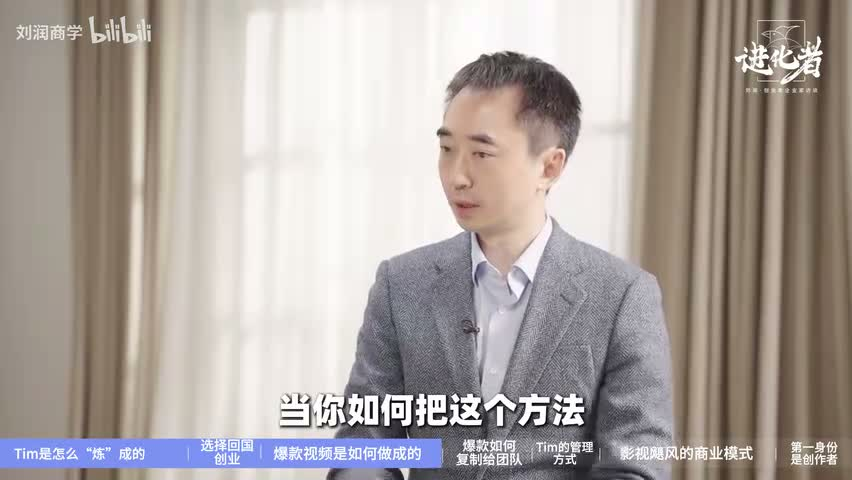
\includegraphics[width=0.70\linewidth,height=0.30\textheight,keepaspectratio]{figures/selected/frame_00-40-38_method_to_team.jpg}
  \caption{从个人方法论转向团队复制：问题的焦点从爆款模型进入组织能力。\protect\footnotemark}
  \label{fig:method-to-team}
\end{figure}
\footnotetext{视频画面时间区间：00:40:37--00:40:44。}

\subsection{复制的边界：Tim 仍然过稿}

团队复制的第一条边界，是最高价值的视频仍要有人承担终局判断。Tim 的回答很清楚：他至少会过稿，未必亲自深度参与每一个制作环节；同时，他也意识到个人投射过重会让每个人身上都刻上自己的影子，这会偏离他的目标。\footnote{源时间：00:40:48--00:41:05。} 这句话的管理含义很重要：团队需要标准，也需要每个创作者形成自己的判断肌肉。

所谓“过稿”，在这里可以理解成一个创意质量闸口。编导可以提出选题、写脚本、组织素材，制片可以安排预算、周期和外景条件，后期可以完成剪辑与节奏，但超级爆款仍要回到几个底层问题：

\begin{enumerate}
  \item 这条内容能否带来快乐，是否具有分享时的轻松感、兴奋感或幽默感？
  \item 它有没有知识增量，观众看完后能否复述一个新信息或新视角？
  \item 它能否触发共鸣，让观众把自己的经历、愿望或情绪投射进去？
  \item 它的节奏是否能支撑从开场、铺垫、转折到结尾的观看动力？
\end{enumerate}

短视频或常规内容可以把某一个属性拉满；超级爆款通常需要多项同时成立。\footnote{源时间：00:41:07--00:41:27。} 因此，方法复制要让每个岗位在自己的环节里看见这些问题，同时避免把每个人塞进同一套模板。编导看选题和脚本，制片看可执行性和风险，后期看节奏与情绪曲线，Tim 的过稿则负责把分散判断重新校准到作品整体。

\subsection{内容矩阵：专业/大众与长/短视频}

当团队达到 100 多人，内容公司无法只围绕单一账号运转。Tim 介绍，团队总共 100 多人，做内容的人差不多 60 多人，其中编导约 20 位，制片约 10 位，剩余是技术型工种，并统一纳入企划与内容相关部门。\footnote{源时间：00:41:33--00:41:53；00:46:12--00:46:24。} 这组数字说明，影视飓风的生产单元已经从个人频道进入组织型内容工厂。

Tim 用一个二维矩阵组织账号和内容定位：一条轴是专业与大众，另一条轴是长视频与短视频。\footnote{源时间：00:41:57--00:43:29。} 这个矩阵的价值在于让团队知道“该做什么”和“用什么成本结构做”。

\begin{table}[htbp]
  \centering
  \caption{内容矩阵：用账号定位约束团队分工}
  \label{tab:content-matrix}
  \begin{tabular}{lll}
    \toprule
    维度 & 代表内容 & 协作含义 \\
    \midrule
    专业长视频 & 影视飓风评测、大型项目、离谱挑战 & 高投入、高技术密度，需要编导、制片、技术协同 \\
    大众长视频 & 一点点不一样、自然科学、人文发现、动物拍摄 & 需要外景、专业顾问、长期题材储备 \\
    大众短视频 & 公司团队 VLOG、氛围与社群内容 & 轻量、高频，强化公司人格和社群连接 \\
    专业短视频 & 短片、短剧与行业热点项目 & 需要明确类型能力和快速试错 \\
    \bottomrule
  \end{tabular}
\end{table}

矩阵背后有一个商业现实：单个频道的广告营收有上限，内容公司需要多个内容产品承接不同受众和不同收入结构。\footnote{源时间：00:42:04--00:42:21。} 这也是组织复制必须面对的资源约束。长视频投入常是短视频的 5--10 倍，尤其是专业长视频和大众长视频，拍摄、交通、设备、安全、专家沟通都会显著抬高成本。\footnote{源时间：00:43:21--00:43:29。}

\subsection{工业化协作：创意需要角色、接口、反馈和约束}

本章的核心概念是“工业化协作”。它指的是把内容生产拆成若干可协作岗位，让创意、脚本、制片、拍摄、技术、后期、发布和复盘形成一条稳定链路。它像高级餐厅从主厨单店扩张到多店经营：口味判断仍然重要，菜单、采购、备料、出餐节奏、成本核算和顾客反馈也必须被拆成明确接口。内容公司同理，创意判断依然在场，协作链路负责把判断放大到更多项目。

从第一性原理看，创意工作的难点来自高度不确定性。观众会不会被打动，天气会不会改变，设备能否承受外景，专家表达能否转化成大众叙事，平台节奏会不会改变，这些都无法在开拍前完全算准。团队化解决的基本问题，是把一个人的大脑压力分解到多个专业单元：

\begin{itemize}
  \item \textbf{创意判断}：有人负责选题价值、情绪方向、知识密度和节奏感。
  \item \textbf{角色分工}：编导、制片、技术、后期、专家顾问等岗位各自承担明确风险。
  \item \textbf{协作接口}：脚本交付标准、预算边界、拍摄清单、素材命名和过稿节点要能连接起来。
  \item \textbf{反馈机制}：成片复盘、数据回看、观众反馈和知识沉淀要进入下一轮项目。
  \item \textbf{资源约束}：预算、周期、体力、安全、商业收入上限和团队人数必须被看见。
\end{itemize}

这组拆分比临时公式更直接。团队复制的瓶颈通常出现在某个环节缺失：只有创意判断，项目会卡在执行；只有岗位分工，作品容易失去灵魂；只有自由环境，结果可能漂移；只有过程控制，创意波动又会被压死。

\begin{figure}[htbp]
  \centering
  
\includegraphics[width=0.86\linewidth,height=0.42\textheight,keepaspectratio]{figures/generated/fig_team_industrial_chain.pdf}
  \caption{团队工业化协作链路：编导、制片、专职人才与复盘共同把个人方法变成组织资产。教学化生成图，综合自 00:27:07--00:28:12 与 00:41:30--00:46:38。}
  \label{fig:team-industrial-chain}
\end{figure}

\begin{importantbox}{团队复制成立的条件}
一个个人创作方法能够进入百人团队，至少要满足五个条件：第一，核心判断有人负责，Tim 仍然在关键稿件上把关；第二，岗位分工足够清楚，编导、制片、技术和专家知道各自承担什么风险；第三，协作接口稳定，脚本、预算、周期、素材、过稿和复盘都有可交接的标准；第四，反馈能沉淀，团队能把一次项目里的教训转成下一次项目的知识；第五，资源约束被公开看见，长视频的高投入、外景风险和商业上限都进入决策。
\end{importantbox}

\subsection{冰岛火山案例：专精化招聘从风险里长出来}

冰岛火山案例说明，工业化协作有具体代价。Tim 讲到团队原本应有更多人去冰岛，因签证问题最后只有少数人前往；他们背着约 30 公斤设备走了约 20 公里山路，到山上拍到火山后，夜里温度从 14 度迅速降到零下 5 度，风很大，衣服不够，团队出现失温风险，其中有人甚至开始出现幻觉。\footnote{源时间：00:43:31--00:45:04。} 这个案例很硬：一条好看的大众长视频，背后可能是设备重量、路线规划、天气窗口、安全预案和体能消耗的复合问题。

从观众视角看，火山节目是“漂亮”“震撼”“稀缺”。从制片视角看，它是预算、签证、设备、路线、保险、天气、人员体能和撤离方案的组合。创意越大，执行风险越高；执行风险越高，岗位专业化越必要。Tim 也因此提到，团队后来意识到只招会拍的人还不够，需要生物背景、户外经验，以及懂具体领域的编导或人才。\footnote{源时间：00:45:07--00:46:12。}

这一点尤其值得内容创业者警惕：当题材从室内评测扩展到自然科学、人文发现和野外项目时，“会拍”只是最低门槛。真正决定作品上限的，是能否把专业知识转成可信叙事，把现场风险转成可执行计划，把专家表达转成观众能理解的发现。Tim 对“一点点不一样”的定位也体现了这种边界意识：他们讲述发现，请行业里真正厉害的专家来讲，避免用创作者自己的嘴去冒充专业判断。\footnote{源时间：00:45:43--00:46:07。}

\subsection{产品团队与公司内创业：让内容公司多一个增长引擎}

内容团队之外，Tim 还提到产品团队有 20 多人，负责电商产品，也在研发 iPhone 配件等自有产品。\footnote{源时间：00:46:24--00:46:32。} 这部分看似偏商业，其实仍属于团队复制问题。原因很现实：如果一家内容公司只依赖频道广告，营收上限会限制内容投入；如果产品线能够跑出来，内容团队就有机会获得更稳定的资源供给。

Tim 把这件事称作一种赌注：未来有没有可能减少对频道广告赚钱的依赖，并用产品收入养活内容团队。他也承认这很难，目前没有先例。\footnote{源时间：00:46:32--00:46:42。} 这种说法很清醒。产品团队、行政支持和孵化小组共同构成“公司内创业”的结构：每个小组都像一个小型实验单元，在公司品牌、流量、供应链和内容理解的基础上寻找新的业务可能。

这里的未知风险同样需要说透。内容团队擅长注意力、叙事和观众信任；产品团队还要面对供应链、库存、售后、毛利、复购和渠道效率。二者共享品牌资产，能力结构却有明显差异。公司内创业的价值在于让团队可以用小单元试错；它的风险在于任何产品失败都会消耗现金、管理注意力和观众信任。

\subsection{Context vs Control：自由环境要用结果负责}

本章最后回到文化。Tim 说，他很重视公司伙伴，认为一些老式企业更重视 Control，也就是控制；而他更看重 Context，也就是实际内容、产出和情境供给。他把焦点放在周期结果上，成员在周期内可能打游戏，创意也会波动；好的环境可以提供，最终结果必须好。\footnote{源时间：00:47:41--00:48:12。}

\begin{knowledgebox}{Context vs Control}
Control 指过程管束，例如打卡、审批、动作监控和固定流程；Context 指让人能做出好结果的上下文，包括目标、信息、资源、审美标准、团队氛围、时间预算和反馈机制。可以用厨房作类比：Control 像主管盯着厨师每一刀怎么切；Context 像提前讲清菜单定位、食材预算、出餐标准、客人反馈和安全边界，然后让厨师对菜品负责。创意团队需要 Context，因为灵感、选题和脚本会波动；管理仍然需要结果，因为作品最终要接受观众、平台和商业目标的检验。
\end{knowledgebox}

这也是工业化协作最容易被误解的地方。把工业化理解成流程捆绑，会压低创意人员的判断空间；把自由理解成目标缺席，团队结果会漂移。Tim 的管理偏好是减少表层规则，追寻内在结果。他在后文还会继续谈到取消打卡、用量化数据观察结果等做法，这些内容会进入下一章的自由化管理与 OKR。\footnote{源时间：00:49:05--00:49:40。}

因此，本章给出的组织逻辑可以压缩成一句话：用 Context 保护创意波动，用角色和接口降低协作成本，用反馈和资源约束校准结果。这样，团队才能在不抹平个人判断的前提下，把 Tim 的方法扩展为公司能力。

\subsection{本章小结}

个人创作方法进入百人团队，需要完成三次转换。第一，方法从个人经验转成可讨论的判断标准，例如快乐、知识、共鸣、节奏。第二，作品从个人执行转成工业化协作链路，编导、制片、技术、专家、后期和复盘各自承担不同风险。第三，公司从单一内容团队转成多引擎组织，内容矩阵、产品团队和公司内创业共同对冲频道广告上限。

本章最重要的提醒是：团队复制的目标是放大判断，避免抹掉判断。Tim 仍然过稿，说明创作经验在关键节点仍有价值；专业化招聘、冰岛火山案例和 Context vs Control，则说明经验必须被角色、接口、反馈和资源约束承接。下一章将继续解释：当自由成为组织文化，OKR 和结果指标怎样防止自由滑向失控。
\section{自由化管理与 OKR：让创意自由，也让结果可检验}

本章的结论先说清楚：创意团队可以拥有很大的路径自由，前提是公司必须把目标、结果指标和成本边界讲透。Tim 所说的自由化管理，把组织从个人感觉漂流中拉回目标和结果；它更像给登山队一张清晰地图和一个明确山顶，然后允许不同小队选择各自的路线、装备和节奏。对内容公司来说，这套逻辑可以拆成三句话：路径交给团队，目标由公司讲清，结果用指标和复盘验收。

\begin{figure}[H]
\centering
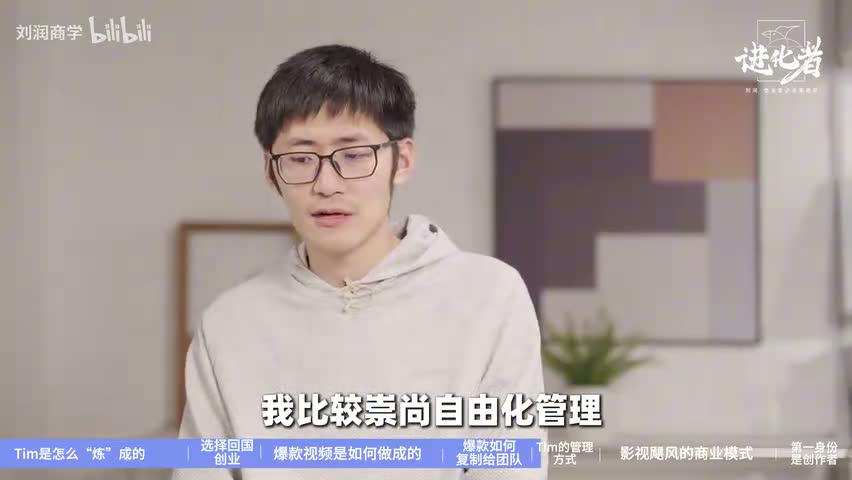
\includegraphics[width=0.70\linewidth,height=0.30\textheight,keepaspectratio]{figures/selected/frame_00-49-41_free_management.jpg}
\caption{自由化管理的起点：让成员自己寻找路径，公司把住整体方向。\protect\footnotemark}
\end{figure}
\footnotetext{视频画面时间区间：00:49:40--00:49:46。}

\subsection{自由化管理：路径放给人，方向收在公司手里}

自由化管理解决的是一个创意组织的根本矛盾：内容质量依赖人的判断、热情和审美，组织规模又要求方向一致、资源可控、结果可复盘。若公司把每个动作都写成流程，创作者会把精力耗在合规动作里；若公司只讲“大家自由发挥”，产出会迅速变成个人偏好竞赛。Tim 的做法是在过程规则上做减法，在目标和结果上做加法：打卡、报销等低价值过程规则可以删减，成员怎样完成任务也可以自主设计，整体方向、周期目标和结果验收必须由公司把住。\footnote{源时间：00:49:05--00:50:08。}

\begin{importantbox}{自由化管理的定义}
自由化管理是“路径自主 + 方向约束 + 结果复盘”的组织方法。个人拥有寻找路径的权利，公司负责定义目标、提供上下文、设置边界、验收结果。它适合创意工作，因为创意的好坏很难靠工时和动作数量直接衡量，却可以通过传播、商业、成本、知识沉淀和团队反馈逐层检验。
\end{importantbox}

这背后的第一性原理很朴素：创意产出像一场开放式解题，管理者很难预先规定每一步。更有效的办法是先让团队理解“为什么做”，再让团队自己回答“怎么做”。在影视飓风的语境里，影响力来自内容被真实观看、真实讨论、真实传播；商业营收来自内容质量、创意权和用户信任；组织迭代来自知识库、反馈表和流程沉淀。自由的价值在于让团队能找到更适合自己的路径，管理的价值在于保证这些路径最后通向同一个目标。

\begin{warningbox}{常见误解：把自由理解成无须负责}
自由化管理最容易失控的地方，是成员只拿走路径自由，回避目标解释、数据复盘和成本约束。真正的自由会减少低价值过程管束，同时增加结果暴露：目标讲清楚，指标可检查，预算有边界，复盘能追问。这样的自由对人要求更高，因为它要求成员证明自己的判断有效。
\end{warningbox}

\subsection{OKR 的底层逻辑：目标来自第一性原理}

OKR 是 Objective and Key Results 的缩写。O 是目标，回答“这个周期到底要成为什么”；KR 是关键结果，回答“怎样知道目标已经接近达成”。一个周期的 OKR 顺序很简单：先确定来自第一性原理的目标，例如“扩增影响力”要服务内容公司的长期竞争力；再拆出可观察、可复盘、和目标有因果关系的关键结果；最后让团队选择行动方案，例如持续稳定内容、冲击爆款、优化转化内容、建设知识库。

\begin{knowledgebox}{OKR 与机械指标的差异}
机械指标像只看体重秤上的数字，短期可以通过脱水、少吃一顿来改变读数；OKR 更像一份体检报告，体重、血压、血糖、心肺能力会互相校验。Tim 反复强调，指标必须逼近底层目标。若目标是影响力，单看粉丝数会诱导买粉；若同时看榜单竞争力、完播率、进入热门的时间、总播放量和内容转化，造假空间会明显变小。
\end{knowledgebox}

买粉为什么会被影响力逻辑淘汰？原因在于买粉只改变了表层计数，内容被真实消费的因果链仍然停在原地。真正的影响力要看五类证据：有效粉丝是否会观看、互动、转化或长期记住创作者；真实播放是否来自真实观看需求；完播率是否说明内容持续抓住注意力；主动传播是否包含转发、讨论、收藏和复述；平台竞争指标是否体现内容进入更大的注意力市场。

当购买粉丝上升，真实播放、完播率、主动传播和平台竞争表现没有同步改善，影响力几乎没有增加。Tim 说“买粉最快”，也正是在指出单一数字会诱导团队走向虚假达成；真正的 KR 要把团队逼回内容质量、平台竞争和用户反应。\footnote{源时间：00:50:08--00:51:31。}

\subsection{三类 OKR：影响力、商业营收、组织迭代}

Tim 展开的 OKR 样例很有教学价值，因为它把内容公司看成三层系统：第一层争夺影响力，第二层把影响力转化为可持续收入，第三层把经验沉淀成组织能力。三层都要被衡量，少一层都会出问题：只有影响力会让公司现金流脆弱，只有收入会消耗用户信任，只有内部流程会离观众越来越远。\footnote{源时间：00:52:11--00:54:40。}

\begin{figure}[htbp]
\centering

\includegraphics[width=0.86\linewidth,height=0.42\textheight,keepaspectratio]{figures/generated/fig_okr_three_layer_matrix.pdf}
\caption{OKR 三层目标矩阵：影响力、商业营收、流程迭代。教学化重绘，综合自 00:49:40--00:54:20。}
\end{figure}

第一类是影响力目标。一个周期内，影视飓风希望进一步扩增影响力，KR 包括三个月增粉约 50 万、进入全站排行榜前 20 的内容达到 3 条、至少有 1 条成为榜一。这里的关键点在于，榜单指标比纯播放或纯粉丝更接近“平台内竞争力”。榜一意味着内容在一个更大的注意力市场里获胜，属于超级爆款的信号。

第二类是商业营收目标。Tim 提到周期内要达到几百万毛利，同时自有服装销售 4 万件以上。服装目标的含义并不只是卖货数字，它还在测试自有品牌认知：用户是否愿意把对内容的信任迁移到产品上。短期可以不把利润最大化放在第一位，先验证用户认知和单量，这是一种商业假设验证。

第三类是组织迭代目标。公司内部知识库评分要达到 80 分以上，季度深度反馈处理达成率要达到 90\% 以上。这类 KR 看起来缺少播放量刺激，却决定公司能否从“靠少数人硬扛”走向“让新人也能理解系统”。新员工能否看懂知识库、员工尖锐反馈能否得到答复，都是组织能力的真实压力测试。

\subsection{成本与制片：自由要有预算边界}

自由化管理还必须面对一个冷酷事实：高质量视频会烧钱。Tim 说，一条好视频今天的成本大约可能达到 50\% 左右，早期甚至出现过倒亏十几万也要做一期内容的情况。真正的问题有两层：贵，以及贵得是否有效。缺少制片人和预算结构时，编导的创作冲动可能持续追加场景、灯光、人员和周期，最后把钱花在提升观众感受很弱的地方。\footnote{源时间：00:55:07--00:55:44。}

制片约束的价值，可以用一个简单不等式来理解。这是本版保留的少数公式，因为它表达的是预算决策阈值：新增投入至少要换回等量新增价值。

$$
\Delta V_{\text{观众}} + \Delta V_{\text{品牌}} + \Delta V_{\text{团队}} \geq \Delta C_{\text{制作}}
$$

其中：
\begin{itemize}
  \item $\Delta V_{\text{观众}}$：新增投入给观众带来的体验、理解、情绪或记忆增量。
  \item $\Delta V_{\text{品牌}}$：新增投入给甲方或商业合作带来的可信表达和传播价值。
  \item $\Delta V_{\text{团队}}$：新增投入给团队能力、流程经验和知识沉淀带来的收益。
  \item $\Delta C_{\text{制作}}$：新增场景、灯光、置景、人员、交通、周期和管理复杂度带来的成本。
\end{itemize}

当左侧价值低于右侧成本，创意自由就会变成资源浪费。Tim 举了广告制作中的层层成本：一面墙可能两万，搭景可能八万到十万，灯光师、灯具和拍摄组会继续推高单日成本。\footnote{源时间：00:55:52--00:57:04。} 这些细节提醒读者，内容公司管理的对象覆盖点子、预算、周期、供应链、现场执行和结果交付。制片人存在的意义，是把“想拍得更好”翻译成“这笔钱是否值得花、这段周期是否值得延长、这个方案是否能交付”。

\subsection{三方责任：甲方、观众与团队都会验收结果}

内容公司的商业内容还有一层特殊压力：作品发在创作者自己的账号上，观众对创作者的认知往往大于对甲方的认知。传统广告项目里，甲方满意可能就算交付；自媒体商业内容里，甲方付钱、创作者背书、观众评价会同时发生。Tim 与刘润在这一段讨论的“三方”关系，本质上是在说明商业内容的验收标准更复杂：甲方要效果，观众要信任，创作者团队要承担长期声誉。\footnote{源时间：00:57:52--00:58:28。}

这也解释了为什么单独写收入目标会过窄。商业毛利很重要，因为公司要养团队、激励人才、承担项目风险；观众信任同样重要，因为账号的长期价值来自用户愿意继续看、继续相信；团队责任也重要，因为依赖消耗员工热情和无限加班会使增长透支。自由化管理一旦进入商业场景，就要同时回答三个问题：

\begin{itemize}
  \item 对甲方：内容是否真实传递了产品或品牌的价值，并避免只完成曝光动作。
  \item 对观众：内容是否仍有观看价值，是否守住账号信任。
  \item 对团队：项目成本、周期和复盘是否让组织下次做得更好。
\end{itemize}

Tim 对家庭背景争议的回应，也应放在这个责任框架里理解。他承认父亲在理念上给了自己很多帮助，例如格局、面对人性、处理公司底层逻辑；同时把直接资金帮助和理念帮助作了区分，前者力度低于外界想象，后者对公司治理影响很深。\footnote{源时间：00:58:48--00:59:41。} 这一段对管理主题的意义在于：组织长期运行最终要回到责任，创作者要对团队负责，公司要能挣钱、能激励优秀人才、能继续向前。

\subsection{本章小结}

第四章的核心可以概括为三句话。第一，自由化管理把过程控制降到必要水平，把目标、上下文和结果验收提高到中心位置。第二，OKR 的价值在于把“想要影响力、收入和组织能力”拆成可检验的 KR，并用多指标嵌套降低买粉、刷量和形式主义的空间。第三，创意自由必须接受成本、制片、甲方、观众和团队责任的共同约束；少了这些约束，自由会快速滑向失控。

所以，适合内容公司的自由，核心在于三件事：公司把方向讲透，把指标设准，把成本边界划清，然后让真正懂内容的人去找到路径。能做到这一点，创意自由才会变成组织能力，并避免沦为一次次消耗预算和信任的个人冒险。
\section{商业化：内容公司的三方金字塔}

内容公司的商业化，第一原则是守住三方价值：甲方获得真实有效的品牌表达，创作者愿意为作品署名，观众觉得自己看到了值得信任的内容。Tim 在这一段访谈里把影视飓风的收入说得很直接：广告、商业服务/直播、电商三块构成现金流；真正难的地方在于，钱进入内容之后，内容还要像作品，不能退化成一次投放任务。

\begin{figure}[H]
\centering
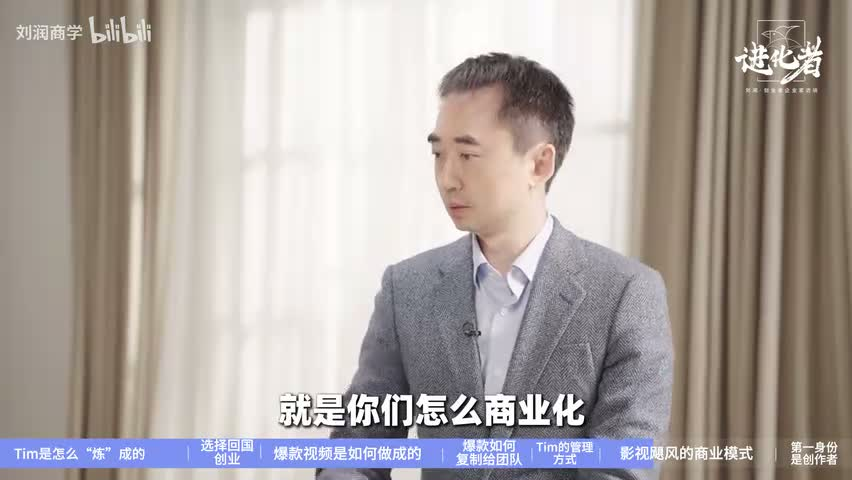
\includegraphics[width=0.70\linewidth,height=0.30\textheight,keepaspectratio]{figures/selected/frame_00-59-56_commercialization_question.jpg}
\caption{商业化问题：内容公司绕不开的经营命题。\protect\footnotemark}
\end{figure}
\footnotetext{源时间：00:59:55--01:00:04。}

本章只基于 \texttt{work/segments/segment\_05\_commercialization.md} 与已检查图像写作。源字幕是 AI 中文字幕，个别人名、行业词和口语数字可能存在识别噪声；例如“烧麦老师”这一称呼来自 ASR 文本，本章保守沿用，不扩展源外身份信息；“中药部”等明显误识别按上下文校正为“中腰部”。

\subsection{三块收入：广告、商业服务/直播、电商}

Tim 对商业化的拆分很朴素：影视飓风本质上有三块收入，分别是广告、商业服务或直播业务，以及电商。教学上可以把它理解为同一个影响力资产的三种变现接口：广告出售的是品牌与内容场景的连接，商业服务出售的是创意、制作和直播交付能力，电商出售的是自有产品与长期用户关系。

这三块收入背后有一个共同底座，Tim 称为粉丝经济。粉丝经济的关键，是把长期信任、内容调性和传播能力转化为商业机会；把粉丝当作流量矿，会快速透支账号信用。内容公司的收入结构看似分散，底层都依赖同一件事：观众是否愿意继续把注意力交给这个账号，并且是否愿意把这种信任迁移到品牌合作、服务交付或自有产品上。

\begin{figure}[htbp]
\centering

\includegraphics[width=0.84\linewidth,height=0.40\textheight,keepaspectratio]{figures/generated/fig_commercialization_paths.pdf}
\caption{商业化路径：广告、商业服务、电商与创意权。此图为教学化整理，综合自 00:59:55--01:02:28 与 01:07:57--01:10:46。}
\end{figure}

\subsection{创意权决定毛利、议价能力与现金流压力}

广告行业有明显上下游。只负责执行拍摄时，内容公司处在可替代位置：甲方或代理公司已经给出创意，制作方主要拼报价、工期和执行稳定性。Tim 的判断更尖锐：如果拿不到创意权，毛利很难上去，垫款压力会迅速吞掉现金流。

这里的“创意权”包含三层含义。第一，内容公司能提出完整方案，甲方收到的是从洞察到表达的整体设计。第二，甲方愿意相信内容团队对观众心理、节奏和传播方式的判断。第三，项目可以在创意确认之后先拿到预付款，减轻差旅、设备、场地、人员等前期支出压力。

现金流压力来自三件事：拍摄前和拍摄中已经发生的支出越高，压力越大；项目早期收到的预付款越多，压力越小；尾款回收时间、审批周期和付款不确定性越高，风险越大。这能解释 Tim 为什么强调创意权。创意权带来的好处会进入公司的财务结构：预付款越早进入，垫款越少；毛利越高，试错空间越大；甲方越信任方案，团队越能把商业内容做成作品。

\begin{knowledgebox}{背景解释：毛利与垫款}
毛利可以粗略理解为项目收入扣除直接成本后的剩余空间。垫款指公司先替项目把钱花出去，后续再等甲方付款。内容项目常有差旅、设备、人员和后期成本，若毛利低且回款慢，公司看上去接了不少单，账上现金却会被前期支出抽空。
\end{knowledgebox}

\subsection{科沃斯点云故事：商业内容如何同时成立}

科沃斯扫地机器人案例，是本章最关键的商业内容样本。按 Tim 的叙述，影视飓风早已有一个创意：艺术家烧麦老师希望纪念离世的爷爷，想把爷爷的房间留下来；团队需要扫描房间、采集数据，甚至涉及武汉城市空间与点云视觉表达。科沃斯的扫地机器人激光雷达，正好能被真实地用于这个创意。

这个项目的价值在于三条线同时成立。对甲方来说，设备能力被真实使用，品牌露出只占表层；对创作者来说，这个故事有情感、有技术挑战，也有艺术表达空间；对观众来说，内容的主体验是纪念、点云可视化与人的情感，口播退到辅助位置。

\begin{importantbox}{三方商业内容原则}
商业内容要同时回答三个问题：

\begin{itemize}
  \item 甲方是否满意：产品能力、品牌信息和合作目标是否被清楚表达。
  \item 创作者是否热爱：团队是否愿意把审美、技术和情感投入到项目里。
  \item 观众是否喜欢：观众是否获得故事、知识、情绪或审美价值，并愿意承认这是一条好内容。
\end{itemize}

三方价值同时成立时，商业内容才有机会从“投放”升级为“作品”。其中任何一方长期受损，账号的信任资产都会被消耗。
\end{importantbox}

这个三角关系也解释了为什么自媒体商业内容比传统 TVC 更复杂。传统广告的验收重心通常落在甲方，甲方点头意味着交付结束；自媒体账号还要面对观众，观众会把商业内容直接记在创作者身上。商业内容如果让观众感觉被糊弄，伤害会回到账号长期信用。

\begin{warningbox}{风险：观众信任一旦损坏，商业效率会反向下降}
观众信任像账户本金。短期商业化可以提高当期收入，粗糙植入、虚假体验和低质量口播会消耗本金。本金下降之后，广告报价、转化率、评论区氛围和下一条内容的首轮传播都会受影响。对内容公司来说，失去观众信任会从单次项目事故扩大成资产负债表上的隐性亏损。
\end{warningbox}

\subsection{承认昂贵内容失败：创作伦理也要看结果}

Tim 在这一段把话说得很狠：有些内容投入几十万、做了两个月，播放量只有七八十万，没有达到共鸣目标，他会直接判定这期内容失败。这里讨论的是结果责任：播放量只是信号，内容公司真正要面对的是目标有没有达成。团队很辛苦，成本很高，周期很长，这些都无法自动换成观众共鸣。

这条标准对创作者很残酷，也很必要。内容公司最容易给自己找借口：项目难、预算大、团队努力、技术复杂、甲方满意。Tim 的标准把这些理由压回同一个问题：作品有没有打动人，目标有没有达成，观众有没有被说服。

商业闭环也有危险性。访谈中刘润追问：好内容吸引品牌，品牌收入支持好内容，理论上这是一个正循环。Tim 随即指出，这里面没有稳定的直接因果关系。内容做得好，品牌预算也可能收缩；平台分发可能改变；行业投放偏好可能转向直播带货。商业闭环的强弱至少受四个条件共同约束：内容质量与共鸣能力、品牌方可用于投放或合作的预算、平台算法和商业生态带来的分发能力、观众对账号的长期信任。任何一项明显变弱，闭环都会随之变弱。

\subsection{平台风险：里世界、外世界与头部效应}

Tim 用“里世界”和“外世界”解释平台风险。类比来自游戏：玩家在游戏内部打装备、做代练，装备看起来有价格；游戏厂商更新规则之后，原来的装备可能立即贬值。创作者在视频平台里也类似。账号看起来有粉丝、有播放、有商业合作，但上面还有平台规则、推荐机制、广告生态和品牌预算。

\begin{figure}[H]
\centering
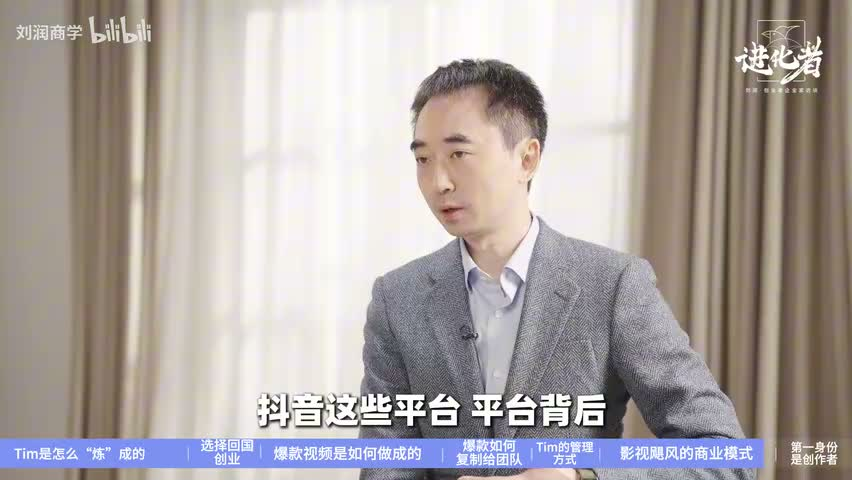
\includegraphics[width=0.70\linewidth,height=0.30\textheight,keepaspectratio]{figures/selected/frame_01-10-00_platform_budget_context.jpg}
\caption{平台和品牌预算变化会改变创作者处境。\protect\footnotemark}
\end{figure}
\footnotetext{源时间：01:09:58--01:10:10。}

这就是中腰部创作者的压力来源。Tim 认为，中腰部博主话语权更小，平台波动会对他们产生巨大影响；品牌总体投放预算减少时，头部账号的预算相对更容易被保护，中腰部批量投放则会优先承压。再加上直播带货把一部分预算拉走，品牌会问一个很现实的问题：中腰部内容投放的转化和认知强化，是否比直播带货更有效？

头部效应因此会越来越强。头部账号既有更高确定性，也能吃到更多预算；更多预算带来更大项目和更强影响力，影响力又让品牌进一步集中。经济学里常把这种现象叫马太效应：已有优势会继续吸附资源。Tim 在 ASR 文本中提到头部可能吃掉很高比例的行业预算，这里应把它理解为口语化的集中度判断；数字层面需要后续人工核验。

\begin{knowledgebox}{概念解释：里世界、外世界与马太效应}
“里世界”指创作者依赖的平台内部生态，包括算法、流量规则、商业产品和推荐机制。“外世界”指平台之外更大的经济环境，包括品牌预算、消费周期、广告市场和技术变化。马太效应描述资源向已有优势者集中的现象，可用一句话概括：越有影响力，越容易获得下一轮影响力资源。
\end{knowledgebox}

\subsection{本章小结}

本章的核心结论是：内容公司的商业化能力，取决于现金流结构、创意权、观众信任和平台环境共同作用。

\begin{itemize}
  \item 收入层面，广告、商业服务/直播、电商是三块主要现金流，底层都依赖粉丝经济与长期信任。
  \item 议价层面，创意权决定内容公司能否摆脱低毛利执行位置，并通过预付款缓解垫款压力。
  \item 作品层面，科沃斯激光雷达点云案例说明，商业内容要让甲方、创作者和观众三方同时获得价值。
  \item 伦理层面，高成本内容没有天然荣誉，结果失效就要承认失败；这是一种对观众、团队和商业伙伴负责的标准。
  \item 风险层面，平台规则、品牌预算转移、直播带货替代、中腰部压力和头部效应，会持续改变内容公司的商业边界。
\end{itemize}

读者应带走一个判断：商业化是内容理想进入现实约束后的经营系统，它会反过来塑造内容选题、制作尺度、组织现金流和账号信任。真正可持续的内容公司，需要在赚钱时仍然证明自己值得被看见、被相信、被传播。
\section{创作者身份与未来：从“做视频”到“输出打动人心的作品”}

本章先给结论：Tim 在公司化之后重构身份的顺序，是把“创作者”放在最高位，再把管理者、艺人/表演者、产品经理这些角色放到创作使命之下。这个排序决定了他的未来叙事：公司要通过自由文化、本土化组织、持续迭代、商业模式升级和内部人才系统，长期输出能让人燃起来、能走向世界、能打动人心的作品。\footnote{源时间：01:11:02--01:17:44}

创作者变成公司以后，真正被管理的对象已经扩展为愿景、人才、资源、技术和商业模式的组合。长期作品力来自四个方面：使命方向决定公司愿意为什么投入，迭代速度决定公司能否从失败中恢复，人才与组织系统决定更多创作者能否站出来，商业模式承载力决定高规格作品能否持续支付成本。

\subsection{第一身份仍是创作者}

刘润在结尾处把问题问得很直接：现在怎么看待自己的定位，是创作者，还是老板。Tim 的回答也很直接：他认为自己第一身份仍然是创作者。他解释说，自己能带动团队，核心来自享受创作、把激情传递给别人，并且在开心时调动他人的共情；他主动降低了“高深管理术”在自我解释中的权重。\footnote{源时间：01:11:02--01:11:27}

\begin{dialoguebox}{身份排序的原话片段（源时间：01:11:02--01:11:57）}
\textbf{刘润}：你觉得你第一身份是个创作者，还是个老板？

\textbf{Tim}：我认为还是个创作者。本质上我也就是个做创作者的料。我是一个享受创作、能把激情传递给别人的人。

\textbf{Tim}：第一顺位还是创作者，第二顺位是管理者，第三顺位是艺人，第四顺位可能是产品经理。
\end{dialoguebox}

这段对话的教学价值在于，它把身份排序写成了组织设计的入口。第一身份是创作者，意味着公司愿景的源头仍然是作品；第二身份是管理者，说明作品需要团队、流程和结果约束；第三身份是艺人/表演者，说明 Tim 自己也承担镜头前的人格表达和情绪调动；第四身份是产品经理，说明“怪点子”需要落到产品、体验和商业承接上。

\begin{figure}[htbp]
  \centering
  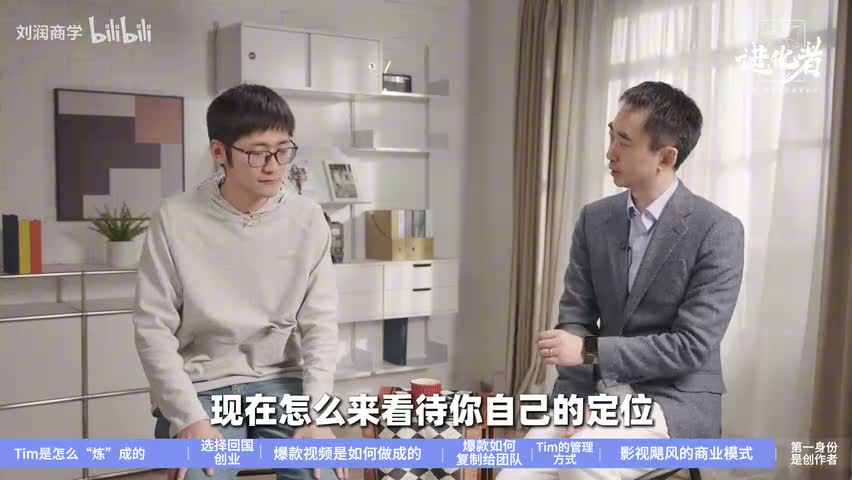
\includegraphics[width=0.70\linewidth,height=0.30\textheight,keepaspectratio]{figures/selected/frame_01-11-03_creator_identity_question.jpg}
  \caption{身份讨论的开场问题：创作者公司化以后，第一身份的排序会影响后续管理、商业与愿景选择。\protect\footnotemark}
  \label{fig:section06-creator-identity-question}
\end{figure}
\footnotetext{视频画面时间区间：01:11:00--01:11:06}

把这四个身份放在一起看，Tim 的角色结构更接近“创作型经营者”。创作者提供情绪燃料和作品判断，管理者把判断交给团队执行，艺人/表演者维持公众表达的感染力，产品经理把创意转换成可被使用、可被购买、可被反复优化的内容产品。前五章讲的是爆款、团队、OKR 和商业闭环；第六章把这些机制收束到一个问题：这家公司最后由什么价值观牵引。

\subsection{Netflix 参照：自由文化需要本土化落地}

刘润提到 Tim 过去说过，希望把自己做成一家像 Netflix 那样的公司。Tim 的解释很清楚：他好奇一家上万人规模的公司，怎样长期产出优质剧集；他认可 Netflix 过去创造了许多优秀内容，也学习其自由文化理念，同时强调不同国家、不同文化需要本土化适配。\footnote{源时间：01:11:57--01:12:37}

\begin{knowledgebox}{Netflix 自由文化在这里指什么}
本章把“Netflix 自由文化”理解为一种组织参照：尽量提高人才密度、给创作者更大自主权、用充分上下文和结果标准替代细碎过程管控。Tim 在访谈里没有展开制度细节，因此正文只使用源内明确出现的“自由文化”和“本土化适配”两个层面，不把外部管理理论强行套入影视飓风。
\end{knowledgebox}

这里的“本土化”很重要。自由文化如果直接照搬，容易变成口号；落在一家中国内容公司里，它必须回答更具体的问题：什么岗位可以高度自主，什么预算需要制片约束，什么内容需要 Tim 亲自过稿，什么 KR 能检验影响力，什么商业内容必须同时对甲方、创作者和观众负责。也就是说，Netflix 提供的是参照系，影视飓风要把它翻译成自己的组织语言。

从前文看，这种翻译已经有几层基础：第三章的编导、制片、专职人才与内容矩阵；第四章的自由化管理和 OKR；第五章的创意权、三方金字塔和平台风险。第六章的 Netflix 参照延续这些话题，回答一个更大的组织命题：创意公司扩张以后，怎样让自由继续服务作品质量。

\subsection{公司使命：无限进步与让中国人燃起来}

当刘润追问未来要把公司带到哪里，Tim 先回到一个经验：很多事情一开始听起来都很离谱，比如 2015 年说想有卫星，后来真的有了卫星。由此，他引出公司的座右铭“无限进步”：只有迭代能与残酷的世界抗争。\footnote{源时间：01:13:11--01:13:38}

\begin{importantbox}{使命、迭代与作品的关系（源时间：01:13:29--01:15:38）}
本章的核心关系可以概括为：使命给方向，迭代给抗压能力，技术和商业模式提供能力底座，作品承担最终的情绪与价值输出。若只保留“让中国人燃起来”这句口号，读者会丢掉机制；若把“无限进步”落实到技术、商业模式和人才系统，使命才有机会变成持续作品力。
\end{importantbox}

“让中国人燃起来”是 Tim 给出的公司使命。他解释这种“燃”来自少年时看热血动漫的感受，也来自对现实压力的观察：许多中国年轻人背负家庭期待、社会机会变化和成熟社会带来的疲惫感。影视飓风能做的事情有限，其中一个具体角色是做“小火花”，让观众看到世界上还有这样的活法、这样的内容，从而对明天多一点期待。\footnote{源时间：01:13:49--01:14:46}

这句话容易被读成鸡汤，所以必须把它拉回内容公司的工作台。“燃”在这里不能停留在单纯口号或宏大词汇里。它更像一种心理能量：观众看见不同活法、不同技术、不同冒险和不同作品后，眼里多一点光，心里多一点行动可能性。第二章的“共鸣”、第五章的“打动人心”，到这里被升级成公司的使命语言。

\begin{warningbox}{愿景最容易变成空口号}
“无限进步”“让中国人燃起来”“向世界输出打动人心的作品”都很大。大愿景一旦脱离机制，就会变成漂亮标语。检验方法很简单：它能否改变选题标准、预算分配、人才培养、技术投入、商业模式和复盘动作。能改变动作，愿景才进入组织；只能写在墙上，愿景就停留在修辞。
\end{warningbox}

\subsection{愿景：媒介会变，打动人心保持底层稳定}

Tim 接着把愿景推到更高一层：以不断迭代的技术和商业模式，向世界输出打动人心的作品。他特别强调，内容和商业模式同等重要，商业模式会随着科技和技术变化而变化；作品形态也会随着 VR、眼镜等媒介变化而变化，视频消费和内容消费方式可能随之改变，“打动人心”仍是底层稳定项。\footnote{源时间：01:14:49--01:15:38}

\begin{dialoguebox}{愿景的原话片段（源时间：01:14:49--01:15:38）}
\textbf{Tim}：以不断迭代的技术和商业模式，向世界输出打动人心的作品，这是我们的底层内核。

\textbf{Tim}：内容和商业模式是同等重要的。商业模式会随着科技和技术的变化产生变化。

\textbf{Tim}：作品形态会变化，随着 VR、眼镜上来，内容消费都会变化；打动人心是底层的。
\end{dialoguebox}

这段话把“内容理想”和“经营现实”接在一起。内容公司同时面对两条约束：作品缺少现金流会受限；商业模式消耗作品信用会伤害观众信任。Tim 选择把两者并列，说明他理解内容公司的底层矛盾：作品需要商业供血，商业需要作品信用，技术变化又会不断改写两者的连接方式。

\begin{figure}[htbp]
  \centering
  
\includegraphics[width=0.70\linewidth,height=0.30\textheight,keepaspectratio]{figures/selected/frame_01-15-05_content_business_equal.jpg}
  \caption{Tim 将内容与商业模式并列，提示读者：愿景要靠作品价值和经营结构共同承载。\protect\footnotemark}
  \label{fig:section06-content-business-equal}
\end{figure}
\footnotetext{视频画面时间区间：01:15:00--01:15:09}

VR、智能眼镜和新型显示设备只是例子。更普遍的规律是，媒介一变，叙事节奏、交互方式、成本结构、分发平台和商业模型都会跟着变。短视频改变了信息密度，直播改变了销售链路，VR 和眼镜可能改变沉浸感与第一视角表达。对影视飓风这样的公司来说，真正稳定项落在让观众产生情绪触动、价值认同和记忆点的能力上。

\begin{figure}[htbp]
  \centering
  
\includegraphics[width=0.82\linewidth,height=0.36\textheight,keepaspectratio]{figures/generated/fig_mission_iteration_work_relation.pdf}
  \caption{使命 / 迭代 / 作品关系图：使命给方向，迭代提供抗压能力，技术与商业模式支撑作品持续触达人心。图形综合自 01:13:33--01:15:30。}
  \label{fig:section06-mission-iteration-work-relation}
\end{figure}

图 \ref{fig:section06-mission-iteration-work-relation} 把这组关系压缩成一个循环：使命指向“让中国人燃起来”，方法是“无限进步/持续迭代”，能力底座来自技术和商业模式，输出是打动人心的作品；当观众对明天多一点期待，使命又获得新的反馈。这个循环解释了 Tim 谈未来时怎样从“做更大账号”推进到“向世界输出作品”。

\subsection{2028 奥斯卡目标：敢想，也要靠体系搭建}

最后，Tim 给出一个非常高的远期目标：2028 年希望拿到奥斯卡短片奖，或者戛纳、圣丹斯等重要电影节奖项；他强调希望是获奖，提名还不够。他也补充说，长片可能暂时够不到，短片有概率冲击。这一目标延续了早年“星辰大海和奥斯卡”的公司命名想象，也延续了从“放卫星”到真实卫星项目的敢想路径。\footnote{源时间：01:15:41--01:16:34}

这里需要冷静处理。奥斯卡和电影节奖项需要审美、工业、叙事、国际传播和评奖机制共同支撑，喊出目标无法自动缩短距离。Tim 的话真正有价值的部分，在于他马上把目标落回系统：自己未必亲自拍摄那部片子；他的责任是搭建体系，让公司内部有人能够站出来。\footnote{源时间：01:16:34--01:16:44}

这句话完成了从个人创作者到内容公司的身份转换。早期，Tim 是亲自写、亲自拍、亲自学、亲自更新的人；公司化以后，他还要让别人有机会站到作品中心。所谓体系，至少包括五件事：选题机制能发现高价值故事，制片机制能承载高难度项目，人才机制能让年轻创作者成长，商业机制能支付长期投入，文化机制能允许大胆目标出现。

结尾还提到两个未来计划：一个与“船”相关，另一个与太空相关；Tim 没有展开细节，只表示未来两三年可能会看到更有趣、更惊讶、更不可思议的事情。\footnote{源时间：01:16:46--01:17:19} 这些内容适合保留为方向性线索，不能写成已确定项目成果。对读者更重要的启发是：愿景型公司需要保留足够大的想象空间，同时用组织系统把想象转成可执行项目。

\subsection{本章小结}

本章把访谈的最后六分多钟收束成一个身份与愿景模型：Tim 的第一身份是创作者，第二身份是管理者，第三身份是艺人/表演者，第四身份是产品经理。这个排序说明，影视飓风的未来叙事依旧从作品出发，再通过管理、表达和产品化能力把作品放大。

\begin{itemize}
  \item 创作者身份提供源头判断：享受创作、传递激情、调动共情，是 Tim 解释自己能带动团队的核心原因。
  \item Netflix 提供组织参照：自由文化有启发意义，落地时需要本土化，必须被翻译成岗位、预算、目标、复盘和结果标准。
  \item “无限进步”给出方法论：只有持续迭代技术、流程、商业模式和人才系统，内容公司才有抗压能力。
  \item “让中国人燃起来”给出使命方向：作品要让观众看见不同活法，对明天多一点期待。
  \item “向世界输出打动人心的作品”给出长期愿景：媒介和商业模式会变化，触达人心的能力保持底层稳定。
  \item 2028 年奥斯卡短片或重要电影节目标给出远期牵引：真正关键的是搭建体系，让内部创作者能够站出来完成更高规格的作品。
\end{itemize}

至此，全片的主线完成闭环：从表达欲开始，经由爆款机制、团队复制、自由化管理、商业闭环，最后回到创作者使命。内容创业的终点从“把账号做大”升级为建立一个能持续产出好作品、能承受技术与商业变化、能让更多创作者向前站的系统。

\section{总结与延伸}

整场访谈的主线可以压缩为五层系统：创作者表达提供源头能量，爆款机制打开增长半径，组织复制把个人能力变成团队能力，商业承载为长期投入支付成本，使命牵引让公司在技术和平台变化中保持方向。任何一层长期薄弱，系统都会失衡：表达欲无法独自承担百人团队，爆款技巧容易滑向短期流量，组织流程可能挤掉作品情绪，商业收入可能透支账号信用，使命口号也需要资源和执行能力支撑。

\begin{table}[htbp]
  \centering
  \caption{总结主线的源证据锚点}
  \label{tab:summary-evidence-map}
  \begin{tabular}{lll}
    \toprule
    因子 & 章节承接 & 源证据锚点 \\
    \midrule
    创作者表达 & 第一章 & 英国孤立、自学 AE/Premiere、140 多万字小说与每周更新，00:04:21--00:10:27 \\
    爆款机制 & 第二章 & 从 20 万到 45 万粉、快乐/知识/共鸣/节奏四特质，00:18:57--00:21:19；00:33:59--00:35:48 \\
    组织复制 & 第三章 & Tim 仍会过稿，团队有编导、制片、技术与内容矩阵，00:40:37--00:46:38 \\
    商业承载 & 第四、五章 & OKR、成本边界、广告/商业服务/电商三块收入，00:49:40--01:10:46 \\
    使命牵引 & 第六章 & 第一身份是创作者、无限进步、让中国人燃起来、输出打动人心的作品，01:11:02--01:15:38 \\
    \bottomrule
  \end{tabular}
\end{table}

\subsection{从 Tim 个案得到的五条底层经验}

第一，表达欲要靠长期输出变成能力。Tim 从小说、漫画、AE/Premiere 自学、教程发布到设备评测，走的是一条连续训练链。所谓天赋，常常表现为更早开始、更愿意重复、更能从反馈里继续下一次。

第二，爆款要服务更大的议题半径。影视飓风从专业影像评测走向 iPhone、气球、打铁花、卫星和直升机航拍，关键动作是把专业能力放进普通人也愿意讨论的公共议题里。圈层内容维持关系，破圈内容改变高度。

第三，团队复制要保留关键判断。编导、制片、摄影、技术、产品团队可以提高产能和交付稳定性，超级爆款仍需要有人对题材、情绪、共鸣和节奏负责。公司化的目标是放大判断，同时避免把判断抹平成流程。

第四，自由管理要接受结果检验。Tim 讲的自由化管理，核心是路径自主、目标清晰和结果可检验的组合。OKR、成本边界、制片机制、知识库和反馈处理，都是让自由变成组织能力的约束条件。

第五，商业和使命必须同时进入系统。内容公司要养团队、做高投入项目、吸引人才、承受平台变化，就必须有商业模式；与此同时，商业一旦消耗观众信任，作品的长期价值会受伤。Tim 把内容和商业模式并列讨论，说明他已经把创作理想放进经营现实里处理。

\subsection{给内容创作者的实践清单}

读者若要把这套方法迁移到自己的内容项目，可以从下面十个问题开始：

\begin{enumerate}
  \item 这个账号的核心表达欲是什么，创作者为什么愿意连续做三年。
  \item 当前赛道的受众半径有多大，是否存在可以自然扩展的公共议题。
  \item 最近三条内容分别提供了什么快乐、知识、共鸣和节奏设计。
  \item 选题是否包含已经沉淀很久的人、物、景、技术或故事。
  \item 是否有一条内容值得投入远高于日常更新的资源，去冲击频道高度。
  \item 团队里谁负责创意判断，谁负责制片、预算、周期和风险。
  \item 指标是否逼近真实影响力，还是只在粉丝数、播放量等表层数字上打转。
  \item 商业合作是否增强内容完成度，还是只把产品露出塞进作品。
  \item 复盘能否沉淀成知识库，让新人和下一轮项目直接受益。
  \item 长期愿景是否会改变选题、预算、人才和商业模式，而不只是贴在墙上。
\end{enumerate}

\subsection{最后的判断}

这场访谈最有价值的地方，是它把“爆款”从玄学拉回系统工程。爆款依然有运气，平台推荐、社会情绪和外部事件都不可控；可控的部分包括选题半径、真实表达、信息密度、情绪共鸣、节奏测试、团队协作、商业承载和复盘沉淀。

Tim 在结尾谈“无限进步”“让中国人燃起来”“向世界输出打动人心的作品”，这些话很大，也很危险。大话能激励团队，也容易变成漂亮修辞。检验它们的方法只有一个：它们是否持续改变具体动作。若它们能改变下一次选题、下一次预算、下一次招聘、下一次商业选择和下一次作品复盘，它们就进入了系统。

所以，本文最后的结论很直接：爆款内容的短期表象可能像一次侥幸命中，深层结构是创作者、内容产品、组织能力、商业结构和使命牵引共同作用的结果。真正难的地方，也正在这里。单点技巧可以学，系统能力需要长期建设；短期爆发可以发生，长期作品力必须靠一次又一次迭代攒出来。

\begin{importantbox}{读完后的最小复盘}
若读者只带走一张行动卡，可以保留下面六个问题：
\begin{itemize}
  \item \textbf{人}：创作者是否有足够强的表达欲、输入密度和输出纪律。
  \item \textbf{内容}：下一条重点内容是否同时检查快乐、知识、共鸣和节奏。
  \item \textbf{选题}：题材是否借用了已经沉淀很久的人、物、景、技术或故事。
  \item \textbf{组织}：团队是否明确谁负责创意判断，谁负责预算、周期和风险。
  \item \textbf{商业}：商业资源是否提高作品完成度，并守住观众信任。
  \item \textbf{愿景}：长期目标是否已经改变具体动作，例如选题、招聘、复盘和产品投入。
\end{itemize}
这六问分别对应本文六层结构。它们可以作为内容团队每次策划会、复盘会和商业合作评估会的共同检查表。
\end{importantbox}

最后还要避开三类误读。第一，把爆款理解成流量技巧，会低估长期训练、选题半径、题材沉淀和节奏测试。第二，把自由管理理解成轻松管理，会忽略目标、指标、预算和复盘对成员自驱力的要求。第三，把商业化理解成接广告，会漏掉创意权、内容完成度、产品团队、电商承接、平台预算变化和观众信任。读者若只学习表层动作，很容易错过影视飓风真正难复制的系统能力。

\end{document}
